\documentclass{beamer}
\usepackage[utf8]{inputenc}

\usetheme{Madrid}
\usecolortheme{default}
\usepackage{amsmath,amssymb,amsfonts,amsthm}
\usepackage{txfonts}
\usepackage{tkz-euclide}
\usepackage{listings}
\usepackage{adjustbox}
\usepackage[T1]{fontenc}
\usepackage{array}
\usepackage{tabularx}
\usepackage{gvv}
\usepackage{lmodern}
\usepackage{circuitikz}
\usepackage{tikz}
\usepackage{graphicx}

\setbeamertemplate{page number in head/foot}[totalframenumber]

\usepackage{tcolorbox}
\tcbuselibrary{minted,breakable,xparse,skins}



\definecolor{bg}{gray}{0.95}
\DeclareTCBListing{mintedbox}{O{}m!O{}}{%
  breakable=true,
  listing engine=minted,
  listing only,
  minted language=#2,
  minted style=default,
  minted options={%
    linenos,
    gobble=0,
    breaklines=true,
    breakafter=,,
    fontsize=\small,
    numbersep=8pt,
    #1},
  boxsep=0pt,
  left skip=0pt,
  right skip=0pt,
  left=25pt,
  right=0pt,
  top=3pt,
  bottom=3pt,
  arc=5pt,
  leftrule=0pt,
  rightrule=0pt,
  bottomrule=2pt,
  toprule=2pt,
  colback=bg,
  colframe=orange!70,
  enhanced,
  overlay={%
    \begin{tcbclipinterior}
    \fill[orange!20!white] (frame.south west) rectangle ([xshift=20pt]frame.north west);
    \end{tcbclipinterior}},
  #3,
}
\lstset{
    language=C,
    basicstyle=\ttfamily\small,
    keywordstyle=\color{blue},
    stringstyle=\color{orange},
    commentstyle=\color{green!60!black},
    numbers=left,
    numberstyle=\tiny\color{gray},
    breaklines=true,
    showstringspaces=false,
}
%------------------------------------------------------------
%This block of code defines the information to appear in the
%Title page
\title %optional
{ 8.2.56}

%\subtitle{A short story}

\author % (optional)
{Hemanth Reddy-AI25BTECH11018}



\begin{document}


\frame{\titlepage}
\begin{frame}{Question}
Given the ellipse with equation $9x^{2} + 25y^{2} = 225$, find the eccentricity and foci.
\end{frame}



\begin{frame}{Theoretical Solution}
\textbf{Solution:}\\
Step 1: Represent the Ellipse in Matrix Form\\
\begin{align}
   \text{ The given equation of the ellipse is }9x^2 + 25y^2 = 225
\end{align}

\begin{align}
     \text{  The general form of conic is} g(\vec{x}) = \vec{x}^{\text{T}} \vec{V} \vec{x} + 2\vec{u}^{\text{T}} \vec{x} + f = 0
\end{align}
By rearranging the terms:
\begin{align}
    9x^2 + 25y^2 - 225 = 0
\end{align}

By comparing the equation to the general form, we identify the matrices and vectors:
\begin{align}
    \vec{x} = \myvec{ x \\ y }, \quad \vec{V} = \myvec{ 9 & 0 \\ 0 & 25 }, \quad \vec{u} = \myvec{ 0 \\ 0 }, \quad f = -225
\end{align}



\end{frame}

\begin{frame}{Theoretical Solution}
Step 2: Find the Eccentricity\\


The eccentricity $e$ is given by the formula $e = \sqrt{1 - \frac{\lambda_1}{\lambda_2}}$, where $\lambda_1$ and $\lambda_2$ are the eigenvalues of the matrix $\vec{V}$. For our diagonal matrix $\vec{V}$, the eigenvalues are the diagonal entries:
$
\lambda_1 = 9 \quad \text{and} \quad \lambda_2 = 25
$\\
\begin{align}
    \text{Using the formula:}
e = \sqrt{1 - \frac{9}{25}} = \sqrt{\frac{25-9}{25}} = \sqrt{\frac{16}{25}} = \frac{4}{5}
\end{align}


The eccentricity of the ellipse is $\frac{4}{5}$.

Step 3: Find the Foci\\



The foci lie on the major axis, and their location depends on the center and the distance $ae$.



The center $\vec{c}$ of the conic is given by the formula $\vec{c} = -\vec{V}^{-1}\vec{u}$.
Since $\vec{u}$ is the zero vector, the center is at the origin:
$
\vec{c} = \myvec{ 0 \\ 0 }
$


\end{frame}

\begin{frame}{Theoretical Solution}

Foci Location\\

The major axis of the ellipse corresponds to the eigenvector of the smaller eigenvalue of $\vec{V}$, which is $\lambda_1 = 9$. The eigenvector for $\lambda_1 = 9$ is $\myvec{ 1 \\ 0 }$, which lies along the x-axis.

The distance from the center to each focus is $ae$.\\


\begin{align}
    ae = \left( \sqrt{\frac{f_0}{|\lambda_1|}} \right) e
\end{align}
\begin{align}
    \text{where} f_0 = \vec{u}^{\text{T}}\vec{V}^{-1}\vec{u} - f = 0 - (-225) = 225.
\end{align}


\end{frame}
\begin{frame}{Theoretical Solution}
\begin{align}
    ae = \left( \sqrt{\frac{225}{9}} \right) \left( \frac{4}{5} \right) = \sqrt{25} \times \frac{4}{5} = 5 \times \frac{4}{5} = 4
\end{align}


Since the center is at the origin and the major axis is on the x-axis, the foci are at $(\pm 4, 0)$.



The foci of the ellipse are at $(4, 0)$ and $(-4, 0)$.

\end{frame}


\begin{frame}[fragile]
    \frametitle{C Code }
    \begin{lstlisting}

#include <stdio.h>
#include <math.h>

int main() {
    // --- Step 1: Represent the Ellipse in Matrix Form ---
    // The equation is 9x^2 + 25y^2 = 225
    // In matrix form: x^T * V * x + 2u^T * x + f = 0
    // V = [[9, 0], [0, 25]]
    // u = [0, 0]
    // f = -225

    double V[2][2] = {{9.0, 0.0}, {0.0, 25.0}};
    double u[2] = {0.0, 0.0};
    double f = -225.0;

    // --- Step 2: Find the Eccentricity ---
    // The eigenvalues of V are the diagonal elements.
   
        \end{lstlisting}
\end{frame}

\begin{frame}[fragile]
    \frametitle{C Code }
    \begin{lstlisting}

 double lambda1 = V[0][0]; // 9
    double lambda2 = V[1][1]; // 25

    // The eccentricity formula is e = sqrt(1 - lambda1/lambda2)
    double eccentricity = sqrt(1.0 - (lambda1 / lambda2));

    printf("The eccentricity of the ellipse is: %.2f\n\n", eccentricity);

    // --- Step 3: Find the Foci ---
    // The center is c = -V^-1 * u. Since u is the zero vector, the center is at (0, 0).
    double center_x = 0.0;
    double center_y = 0.0;

   
        \end{lstlisting}
\end{frame}

\begin{frame}[fragile]
    \frametitle{C Code }
    \begin{lstlisting}
 // The major axis length is 2*a, where a = sqrt(f0 / |lambda_min|)
    // f0 = u^T*V^-1*u - f = 0 - f = -f
    double f0 = -f; // 225

    // The semi-major axis 'a' corresponds to the smaller eigenvalue (9).
    double semi_major_axis = sqrt(f0 / lambda1); // sqrt(225/9) = sqrt(25) = 5
    
    // The distance from the center to each focus is 'ae'
    double foci_distance = semi_major_axis * eccentricity;

        \end{lstlisting}
\end{frame}

\begin{frame}[fragile]
    \frametitle{C Code }
    \begin{lstlisting}


    // The foci are located on the major axis (the x-axis, corresponding to lambda1)
    printf("The foci are located at (+/- ae, 0):\n");
    printf("Foci: (%.2f, %.2f) and (%.2f, %.2f)\n", foci_distance, 0.0, -foci_distance, 0.0);

    return 0;
}

            \end{lstlisting}
\end{frame}


\begin{frame}[fragile]
    \frametitle{Python Code }
    \begin{lstlisting}
    import numpy as np
import matplotlib.pyplot as plt

def plot_ellipse_solution():
    # Given equation: 9x^2 + 25y^2 = 225
    
    # 1. Find a, b, e, and the foci
    a = np.sqrt(25)
    b = np.sqrt(9)
    
    eccentricity = np.sqrt(1 - (b**2 / a**2))
    
    # Distance from center to foci
    c_foci = a * eccentricity
    
    foci_coords = [(-c_foci, 0), (c_foci, 0)]
    
    print(f"Semi-major axis (a): {a}")
    print(f"Semi-minor axis (b): {b}")
  
      \end{lstlisting}
\end{frame} 

\begin{frame}[fragile]
    \frametitle{Python Code }
    \begin{lstlisting}

  print(f"Eccentricity (e): {eccentricity:.2f}")
    print(f"Foci: ({foci_coords[0][0]:.2f}, {foci_coords[0][1]:.2f}) and ({foci_coords[1][0]:.2f}, {foci_coords[1][1]:.2f})")

    # 2. Plotting
    theta = np.linspace(0, 2 * np.pi, 100)
    x = a * np.cos(theta)
    y = b * np.sin(theta)

    fig, ax = plt.subplots(figsize=(8, 8))
    ax.plot(x, y, label=r'Ellipse $9x^2 + 25y^2 = 225$')
    
    # Plot the foci
    ax.plot(foci_coords[0][0], foci_coords[0][1], 'ro', label=f'Foci')
    ax.plot(foci_coords[1][0], foci_coords[1][1], 'ro')
    
  
      \end{lstlisting}
\end{frame} 

\begin{frame}[fragile]
    \frametitle{Python Code }
    \begin{lstlisting}

  # Annotate the foci and center
    ax.annotate(f'({foci_coords[0][0]:.0f}, {foci_coords[0][1]:.0f})', foci_coords[0], textcoords="offset points", xytext=(-15, 10), ha='center')
    ax.annotate(f'({foci_coords[1][0]:.0f}, {foci_coords[1][1]:.0f})', foci_coords[1], textcoords="offset points", xytext=(15, 10), ha='center')
    ax.plot(0, 0, 'go', label='Center')
    
    # Add eccentricity label to the plot title
    ax.set_title(f'Ellipse with Eccentricity e = {eccentricity:.2f}')
    ax.set_xlabel('x')
    ax.set_ylabel('y')
   
    
    
      \end{lstlisting}
\end{frame} 

\begin{frame}[fragile]
    \frametitle{Python Code }
    \begin{lstlisting}
     ax.grid(True, linestyle='--')
    ax.axhline(0, color='black', linewidth=0.5)
    ax.axvline(0, color='black', linewidth=0.5)
    ax.set_aspect('equal', adjustable='box')
    ax.legend()
    plt.show()

plot_ellipse_solution()
      \end{lstlisting}
\end{frame} 

\begin{frame}{Plot}

\begin{figure}
    \centering
    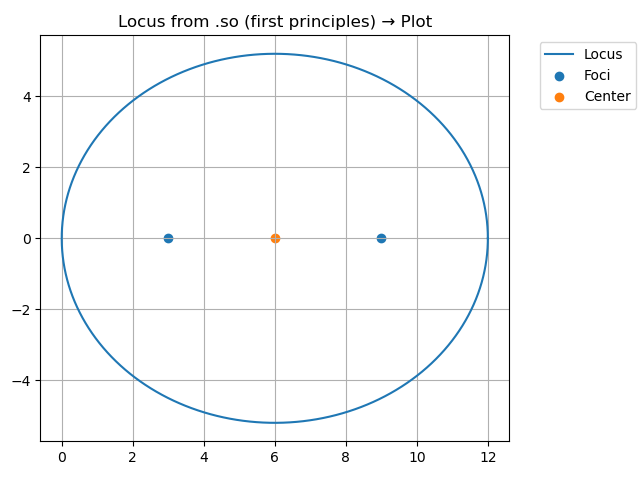
\includegraphics[width=0.8\linewidth]{Beamer/figs/ellipse.png}
    \caption{}
    \label{fig:placeholder}
\end{figure}

\end{frame}


\end{document}